\chapter{Technical Background and Motivation}
\label{sec:state}

% Hier werden zwei wesentliche Aufgaben erledigt:

% 1. Der Leser muß alles beigebracht bekommen, was er zum Verständnis
% der späteren Kapitel braucht. Insbesondere sind in unserem Fach die
% Systemvoraussetzungen zu klären, die man später benutzt. Zulässig ist
% auch, daß man hier auf Tutorials oder Ähnliches verweist, die hier auf
% dem Netz zugänglich sind.

% 2. Es muß klar werden, was anderswo zu diesem Problem gearbeitet
% wird. Insbesondere sollen natürlich die Lücken der anderen klar
% werden. Warum ist die eigene Arbeit, der eigene Ansatz wichtig, um
% hier den Stand der Technik weiterzubringen? Dieses Kapitel wird von
% vielen Lesern übergangen (nicht aber vom Gutachter ;-), auch später
% bei Veröffentlichungen ist "Related Work" eine wichtige Sache.

% Viele Leser stellen dann später fest, daß sie einige der Grundlagen
% doch brauchen und blättern zurück. Deshalb ist es gut,
% Rückwärtsverweise in späteren Kapiteln zu haben, und zwar so, daß man
% die Abschnitte, auf die verwiesen wird, auch für sich lesen
% kann. Diese Kapitel kann relativ lang werden, je größer der Kontext
% der Arbeit, desto länger. Es lohnt sich auch! Den Text kann man unter
% Umständen wiederverwenden, indem man ihn als "Tutorial" zu einem
% Gebiet auch dem Netz zugänglich macht.

% Dadurch gewinnt man manchmal wertvolle Hinweise von Kollegen. Dieses
% Kapitel wird in der Regel zuerst geschrieben und ist das Einfachste
% (oder das Schwerste weil erste).

%\ldots state of the art \ldots

%\todo{write state}

\section{Technical Background}
In this section, we will introduce some basic knowledge 
you need to know in order to better understand the paper. 
Such as Privilege Transitions,Meltdown attack, Spectre attack and sequence files.

\subsection{Privilege Transitions}
Due to security issues, most operating systems now use a protection ring 
mechanism to isolate user-kernel-land. As wiki explained \textquote{A protection 
ring is one of two or more hierarchical levels or layers of privilege within the 
architecture of a computer system. This is generally hardware-enforced by some CPU 
architectures that provide different CPU modes at the hardware or microcode level. 
Rings are arranged in a hierarchy from most privileged (most trusted, usually numbered zero) 
to least privileged (least trusted, usually with the highest ring number). On most operating systems,
 Ring 0 is the level with the most privileges and interacts most directly with the physical 
 hardware such as the CPU and memory.}
In other words, a program running in user space is untrustworthy because it may be 
an attacker. Therefore, CPU and operating system developers proposed protection rings 
to protect critical resources, such as physical memory, device memory, and scheduler information. 
For instance, the Linux operating system in x86 protected mode uses ring 0 for the kernel and ring 3 
for users. Compared to processes in ring 0 that can do anything, processes in ring 3 cannot touch any critical 
resources. In addition, the most important thing is that processes in ring3 cannot change its ring itself. 
Otherwise, it may set itself to ring0 and destroy the kernel space.

If the program wants to communicate with the device, how can it achieve this goal without changing 
itself to ring 0? The answer is Privilege Transitions. To help user-level processes use resources 
in the kernel, the kernel exposes API called system calls to provide various services, as shown in Figure 1. 
Through this API, the kernel can verify requests from user space before providing services. On top of 
improving system security, the protection ring mechanism and system calls make the program in ring 3 
also more flexible. Because the program does not have to worry about overwriting the memory of other 
processes, nor does it have to compete with others for permission to use devices. All this dirty work 
is treated as a request in the kernel and managed correctly by it.

While this mechanism improves system security and the flexibility of user-level processes, 
it also introduces a significant performance penalty. In the following chapter, we will 
analyze the reason for the performance penalty caused by system calls and propose a new 
mechanism to address this issue. 

\subsection{Meltdown attack}

OS security is always a big concern for system engineering. 
Over decades most operating system security methods and theory are based on memory isolation, 
e.g., the protection ring mechanism. But With the discovery of meltdown, all attempting to protect 
OS based on memory isolation and parevirtualized environment are failed.

The Specter set of vulnerabilities does not target specific modern hardware defects, 
but rather refers to the optimization strategy “Branch Prediction” and "Out of order execution" 
commonly used by CPU, combined with the side-channel attacks to access arbitrary secret data.
Hence, it is extremely difficult to achieve a comprehensive defense.

The Meltdown is the simplest and most well-known attack in this series of vulnerabilities. 
In order to explain the principle of the meltdown vulnerability, we need to integrate 
three aspects of knowledge: virtual memory, out-of-order execution, and cache-based side-channel 
attack such as flush and reload.

As we all known, Modern OS is based on virtual memory to fill the gap between 
large program and relative small physical memory and isolate each process from 
each other. In other word, each program has it's own virtual memory space that is 
divided into 2 parts "user space" and "kernel space" , and Virtual pages are mapped 
to physical pages at page size granularity according to page table.. User space can
only be access by program itself, while only process in kernel mode have ability to 
run in kernel space. In order to facilitate the memory access, all physical page can
be mapped into kernel space, e.g., Process in kernel mode can access all data no
matter where it is. In particuler,  Virtual memory are mapped to physical memory 
at page size granularity according to page table. Normally user space and kernel
space virtual memory leverage the same page table to 
convert virtual address to physical address.
 To isolate user and kernel space, there will be 
 a User/Supervisor bit in each page table entry to specify 
 whether user mode can be accessed. The goal of the meltdown 
 is to break the above-mentioned isolation between user mode and kernel mode, 
 and let process in user mode have the ability to access all physical memory.

Meltdown uses a hardware feature called out-of-order execution to 
achieve this goal. The decoded instructions on modern CPUs that support 
"out-of-order execution" are sent to the CPU scheduler. Once the operand 
of an instruction is available, the CPU execution unit will immediately 
execute the instruction regardless of the order in the code. But results of 
each out-of-order executed instruction are back to the user in order of 
instruction fetch. This is called In-Order Commit. In particular,  
all privilege checking and exception handling are processed during 
the Instruction in-Order Commit period. If the privilege checking is 
failed or an exception is caused by one instruction, the result of this 
instruction and the following are dropped, and the CPU rolls back to a sane state. 

While out-of-order code execution brings performance improvements, 
it also brings obvious security drawbacks. The reason comes from 2
 aspects. On the one hand, CPUs can execute instructions before checking 
 their privilege. It means CPU on user mode may execute instructions 
 belonged to the kernel accidentally. On the other hand, the effect of 
 instructions conducted but not committed may stay visible on cache, 
 although the CPU drops the result of that kind of instruction during 
 the in-order commit period.

Since the effect of instructions conducted but not committed remains 
in the cache, in the case of meltdown attack, an attacker could leverage
 the cache to extract confidential and other data that the attacker wants
  to know. This is called cache side-channel attack, more specifically, 
  flush + reload attack. In simple terms, an attacker flushes the cache 
  in advance; after the illegal instruction has been executed, the 
  attacker can judges whether the illegal instruction has accessed a 
  specific piece of data during this period

In summary, Meltdown vulnerability can leak all privileged 
information by exploit hardware feature called out of order execution 
and cache side-channel attack. This vulnerability is dependent to hardware.
 Hence, this attack is highly versatile, and it is extremely difficult to achieve a comprehensive defense.

Kernel developer brings KPTI(Kernel page table isolation) to protect 
the kernel from meltdown attacks. In simpler terms,  Kernel and 
user-level processes have different page tables, which means the 
out-of-order executed instruction on user mode can't touch any memory 
in the kernel because of the different page tables between kernel and user level processes.
\subsection{Spectre attack}

Spectre vulnerability is very similar to 
Meltdown vulnerability. It bases on transient 
execution as well. But compared to transient 
execution in Meltdown vulnerability caused by 
out of order execution,  transient execution 
in Spectre vulnerability is related to branch 
prediction mistraining. 

Since branch instruction may include memory access, 
it may need several clocks to retrieve data from memory.
Hence, CPU is designed to have a branch prediction unit 
to execute branches based on historical branch execution 
speculatively. The branch execution unit has two parts,
Conditional Branch direction predictor and Target address 
predictor. Conditional branch direction predictor is 
in charge of predict whether the condition of one branch is true.
The responsibility of the target address predictor predicts the 
target address of indirect branches.

An attacker can take advantage of this CPU feature and writes many wrong samples into the branch prediction unit in advance so that the branch prediction unit makes an incorrect prediction of the branch that is about to be executed in the victim's process. In this way, the CPU will execute code that should not be executed in advance. Through the above operations, the attacker can force the CPU to access any location in the victim's address space. Although the CPU will eventually write back these codes and execute the correct branch, the results of these code executions will be kept in the cache. Thus, the attacker can read the secrets saved by the victim by viewing the changes in the cache.

In short, The attack process between spectre and meltdown 
is quite similar, except that spectre requires prediction 
mistraining. In particular, in spectre vulnerability attacker
 can only get data that the victim has the right to access.





\section{Related work}
The IO(INPUT-OUTPUT) refers to data transformation
between user processes and various devices.
A complete IO is usually divided into 2 phases: 
privilege transitions between user space and kernel 
space, communication between kernel space and device 
space. In recent years, with the continuous improvement 
of device IO speed, The overhead of IO operations 
in the kernel has became not negligible anymore. 
To address this problem, Clever developer proposed many 
approaches. In this section, we will cover some of them,
which aim for alleviating the IO performance 
bottleneck caused by the kernel

\subsection{VDSO}
Let us first look at vDSO. vDSO stands for Virtual Dynamic Shared Object, 
which accelerates some read-only system calls by mapping pages containing 
relevant information and codes to user space [2].In particular, the pages are 
mapped both to user and kernel space. While the page in the kernel is writable, 
the mapping containing the page in user space is read-only, and the mapping address 
is randomized against the attacker.  vDSO improves IO performance, 
but it also has obvious limitations. That is, all codes and data related to vDSO in 
the user space are read-only. If the program wants to transfer data to the device, 
it can only enter the kernel or try other methods. Therefore, vDSO is still regarded as an 
IO slow path in the communication context between the application and the device

\subsection{IOURING}
\begin{figure}[tbp]
  \centering
  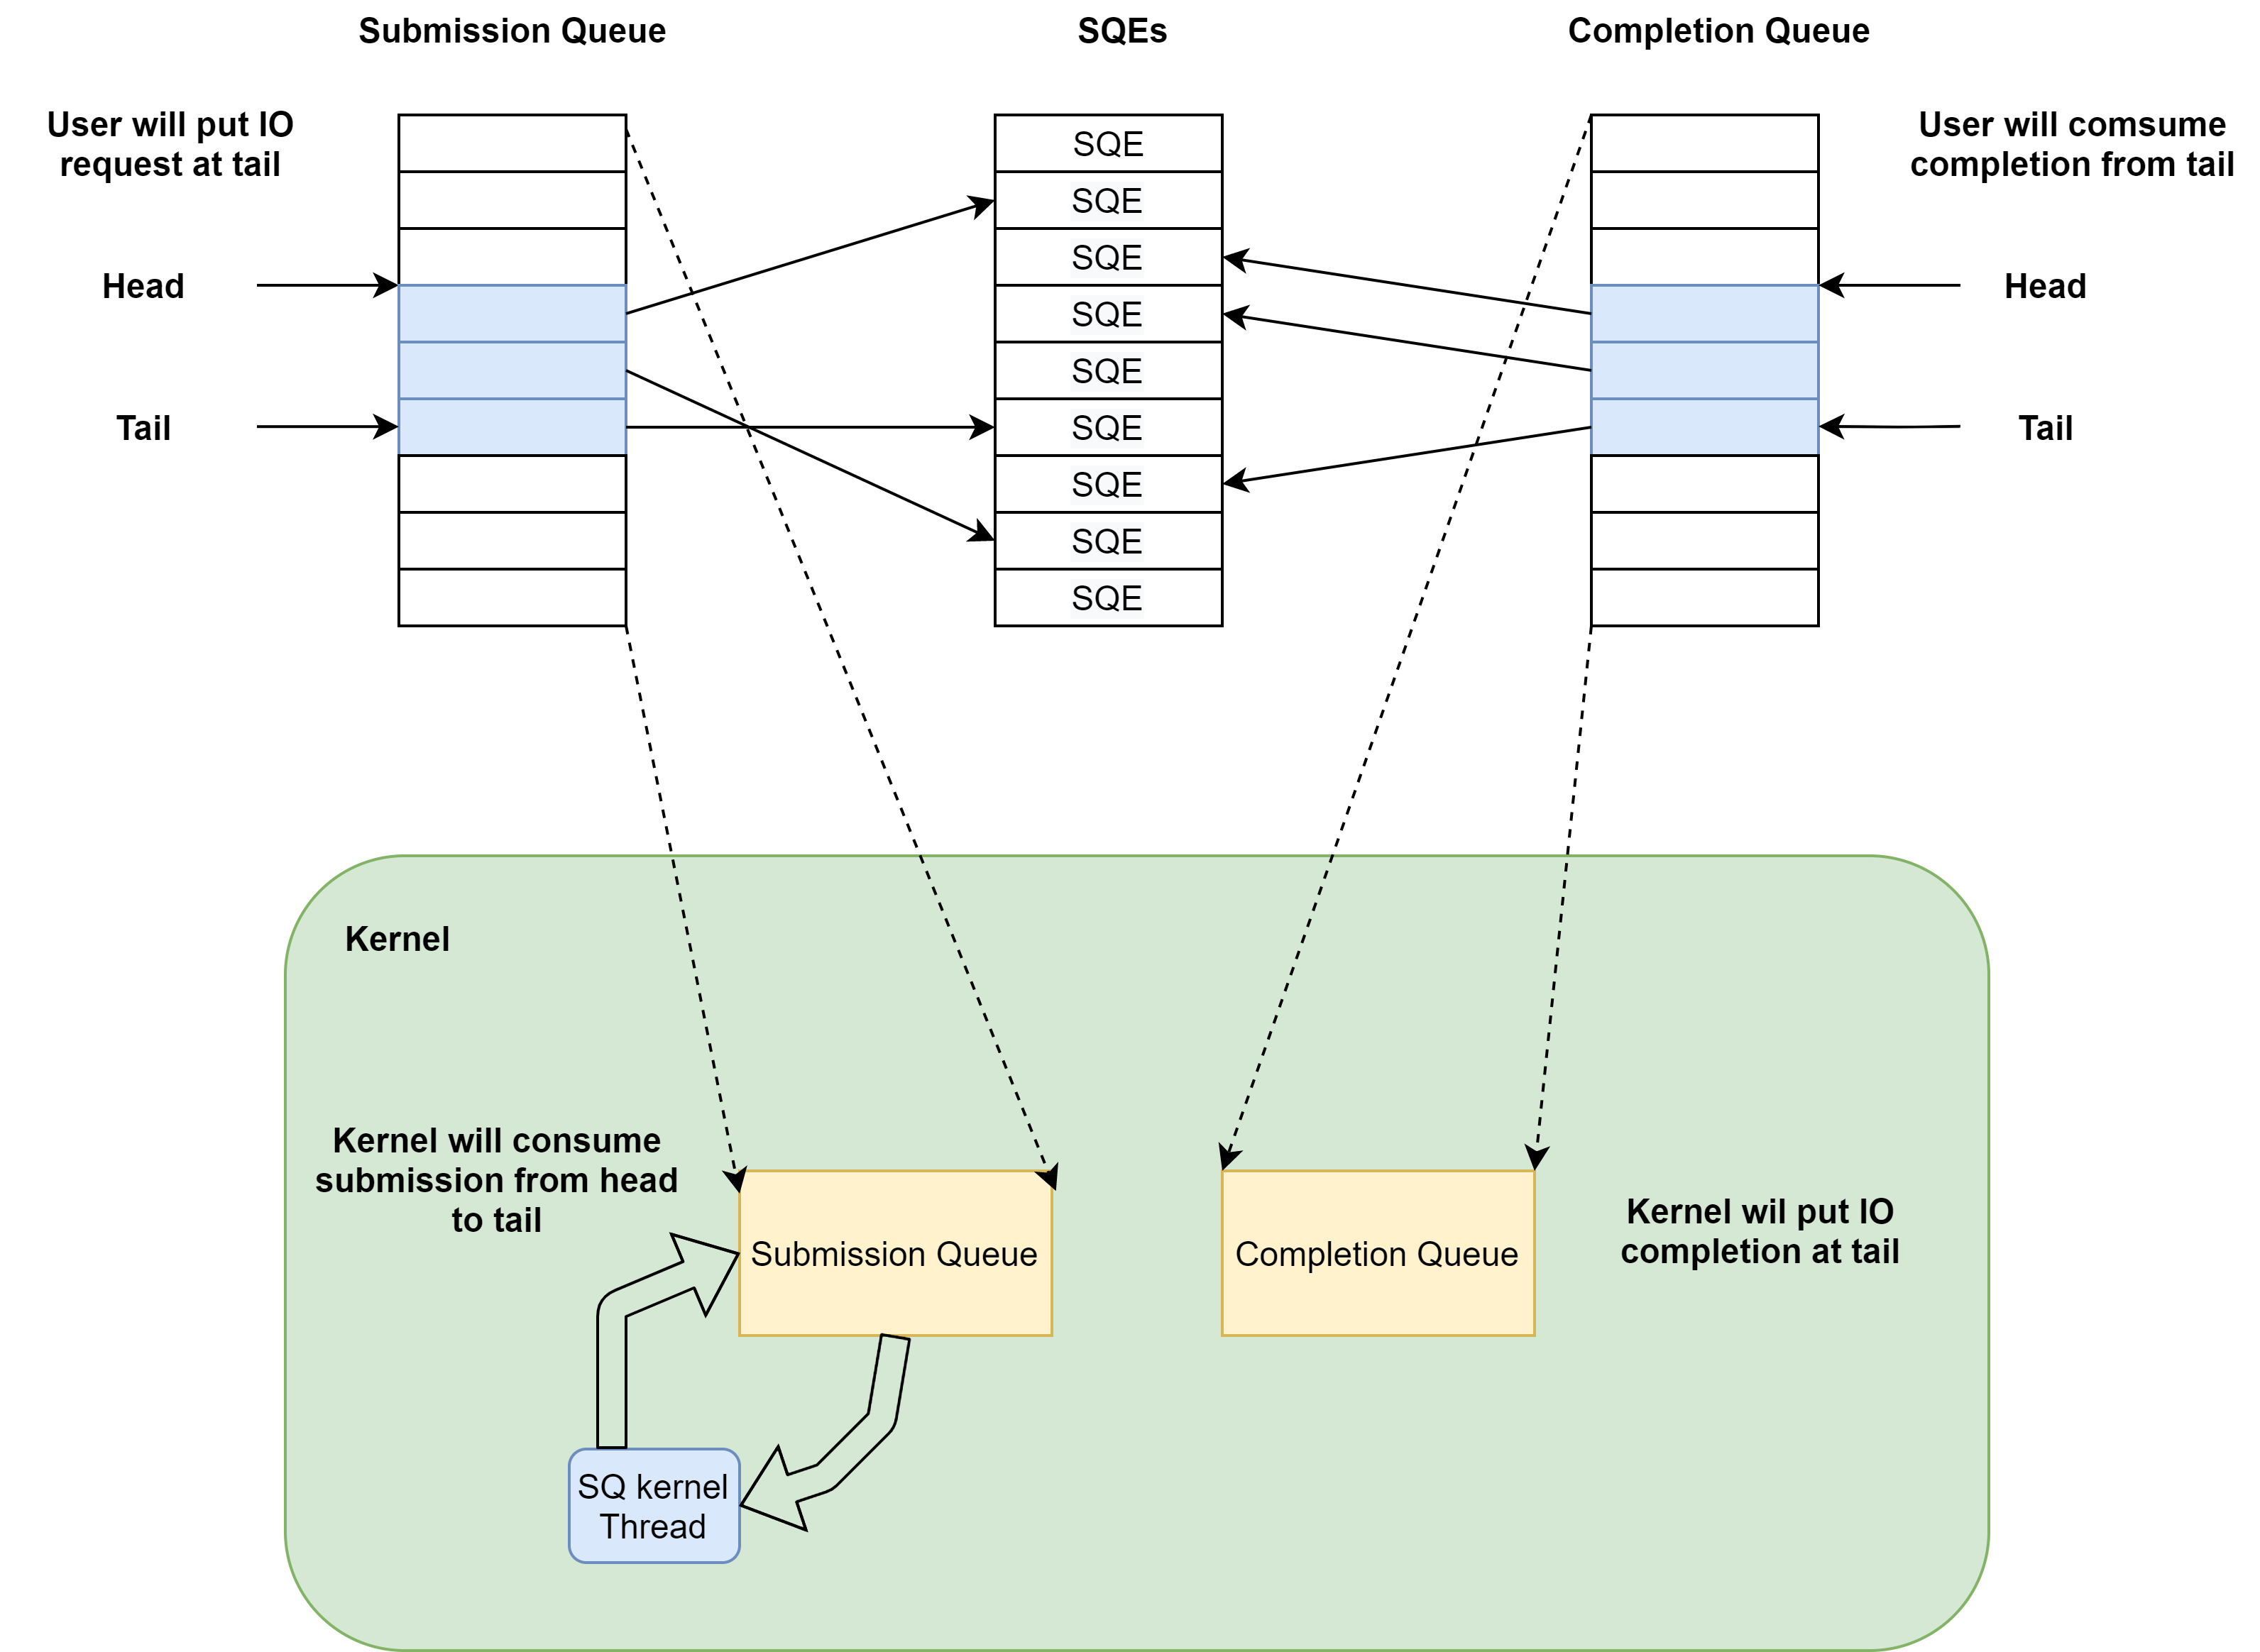
\includegraphics[width=0.8\textwidth]{images/IOURING}
  \caption[Short description]{IOURING}
  \label{fig:IOURING}
\end{figure}
IOuring is introduced in Linux version 5.1 and refers to a new generation of asynchronous I/O API. It offers batch processing and asynchronous I/O submission/completion,  reducing the pressure caused by the user-kernel boundary crossing and eliminating the need for user-kernel boundary crossing in the best case. This is done by entering the fully polled mode that enables an SQ kernel thread to poll the submission queue and to submit any requests found there\cite{Jonathan} automatically.  

In detail, IOuring has three essential components in the fully polled mode. 
Those are submission queue, completion queue, and SQ kernel thread as despite in figure ~\ref{fig:IOURING}. 
Before IOuring operations. User processes need to do three system call to map Submission Queue, 
Completion Queue, and Submission Queue Entries(SQEs)into user space. Submission Queue, Completion 
Queue is a ring buffer, which contains pointers to SQES. 
As for SQEs, it contains either the uncompleted or completed 
IO request. Then user process can directly put the IO request 
into the SQ and get the completed IO request from CQ. Other dirty 
work is finished by SQ kernel thread and kernel handler functions. 
With the help of shared queues between user and kernel space, IOuring 
eliminates the user kernel boundary-crossing for every Io request. 
This has resulted in a noticeable performance improvement.

However, During the IOuring setup stage, IOuring needs at least three system 
calls(6 kernel user boundary crossing). In addition, each executed IO still 
needs to go through multiple layers in the kernel to reach the device finally. 
For instance, a storage-related IO must pass through at least the file system 
layer to arrive at the appropriate device driver layer\cite{Yuhong}. 
Hence, each IO operation still brings noticeable overhead when access new generation devices.


\subsection{OSbypass(DPDK)}
\begin{figure}[tbp]
  \centering
  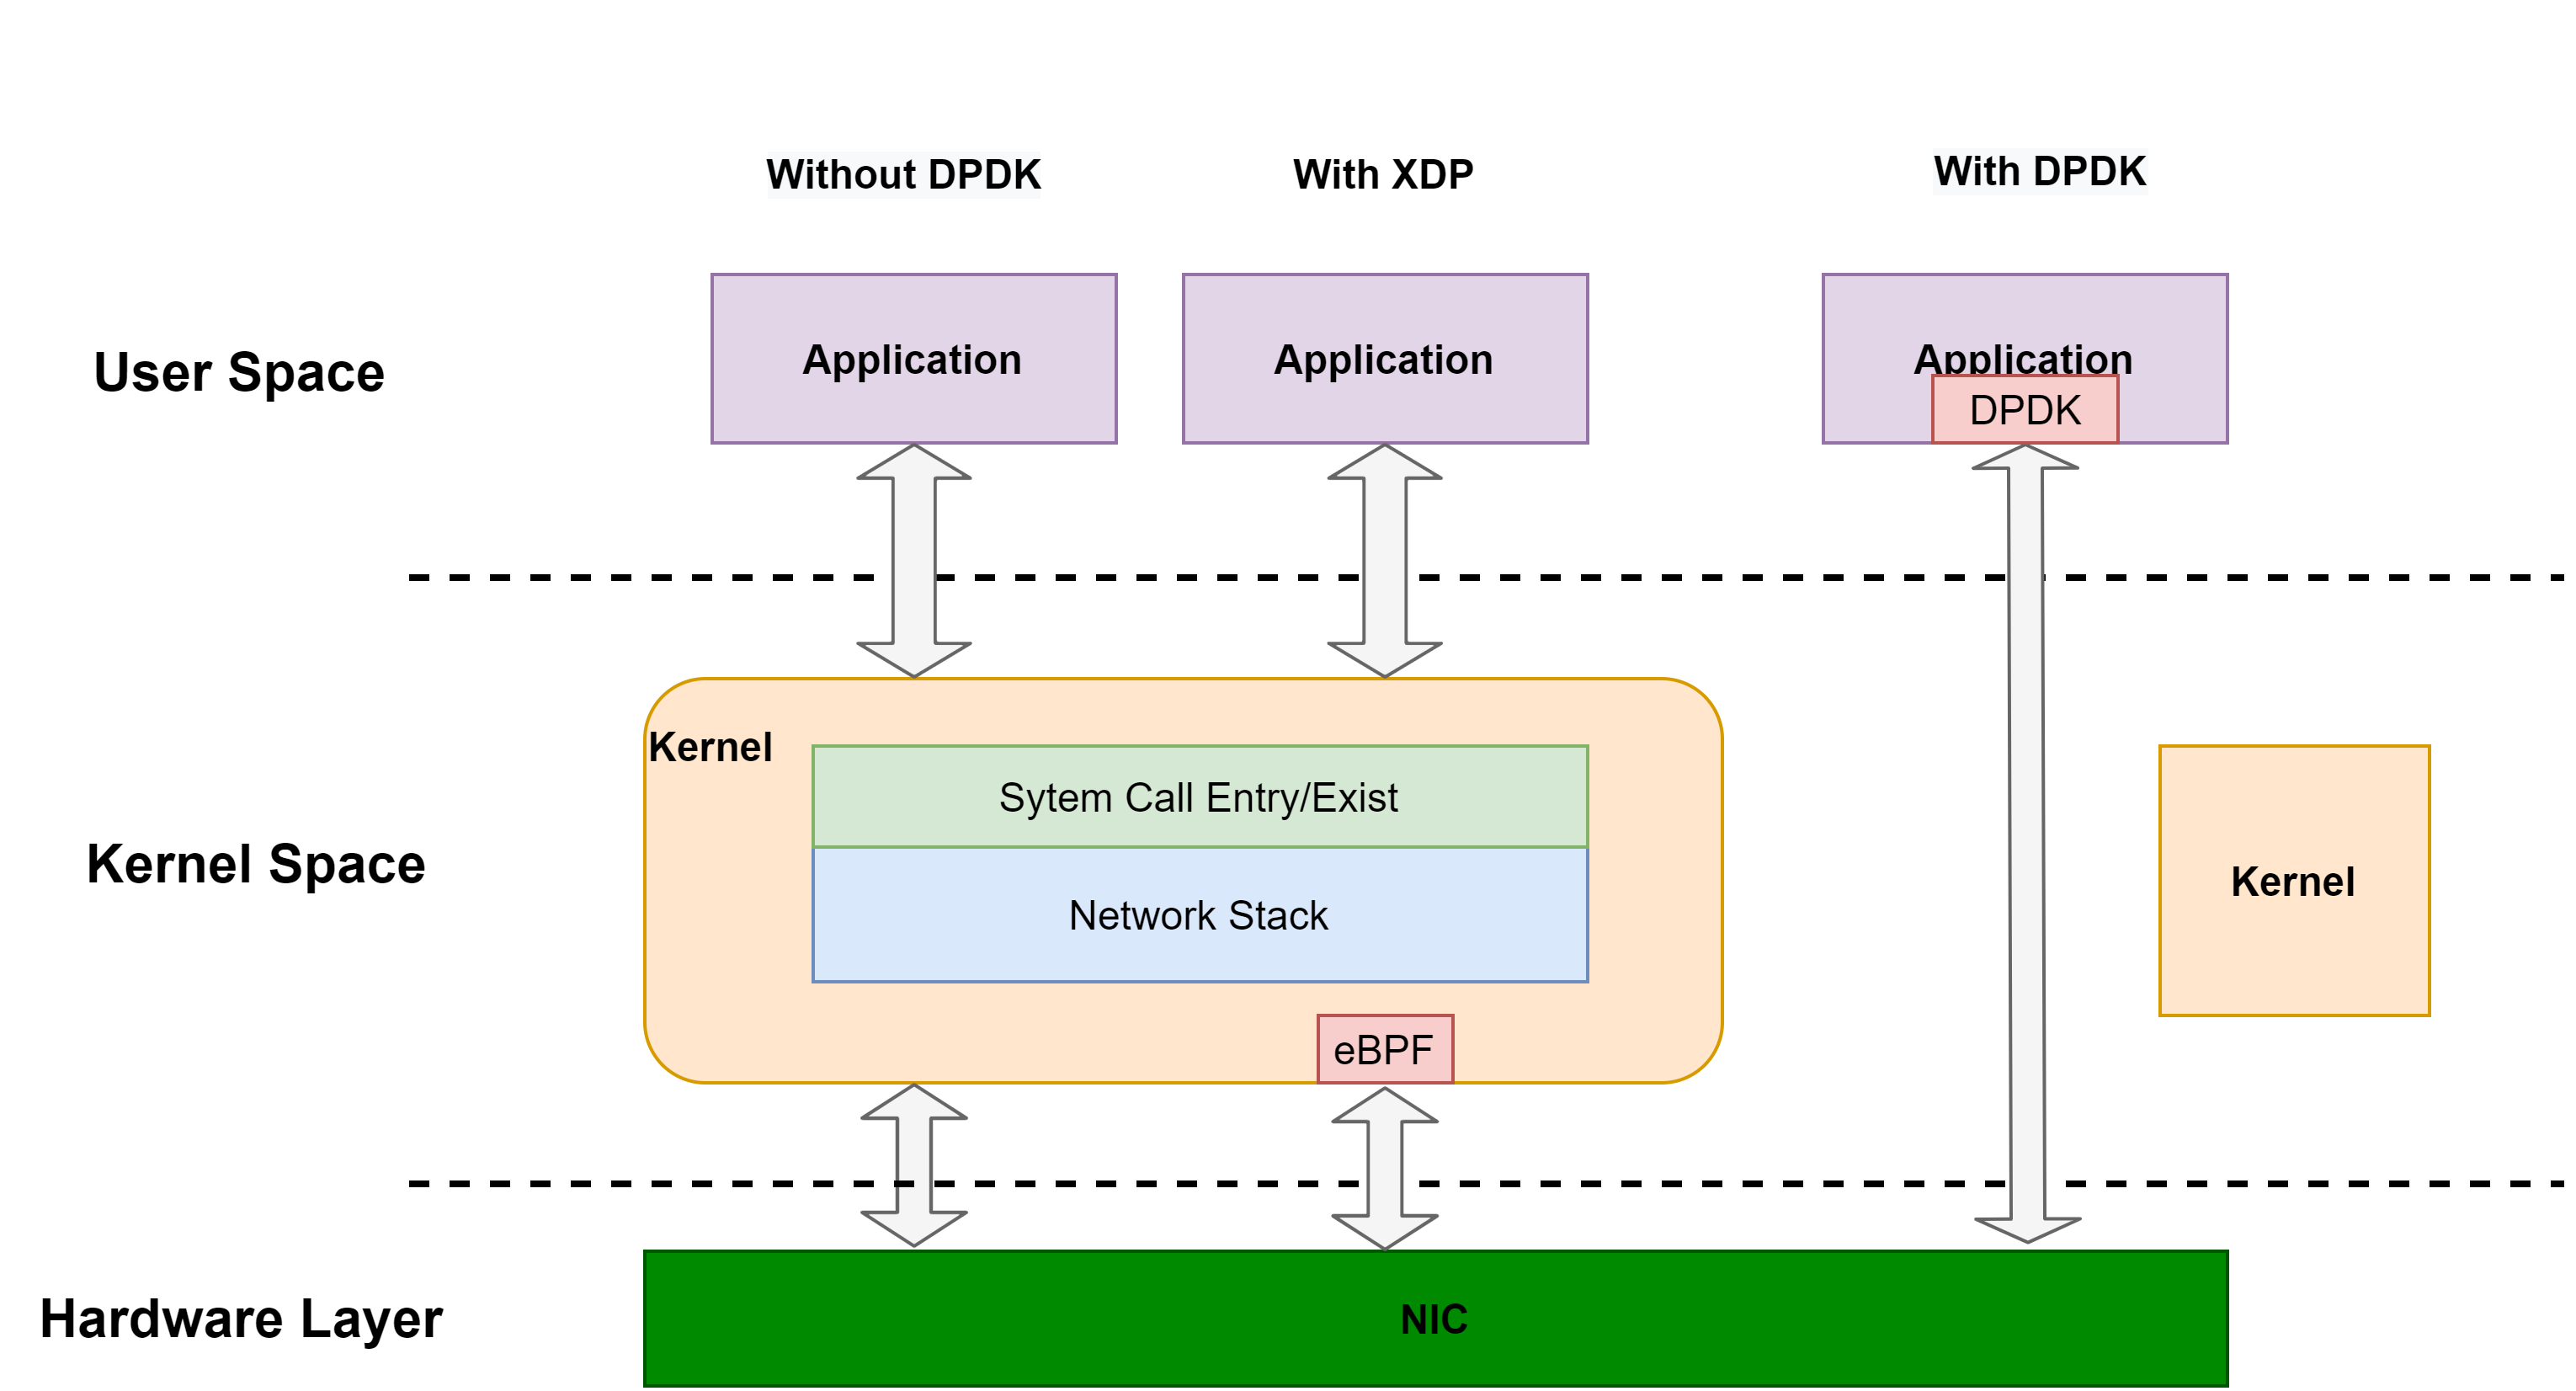
\includegraphics[width=0.8\textwidth]{images/Linux_networking}
  \caption[Short description]{Linux Networking}
  \label{fig:Linux_networking}
\end{figure}

Kernel bypasses, such as DPDK(for intelligent network cards) and SPDK(for NVMe-based storage), 
allow applications to communicate with devices without involving the kernel. For example, as shown in Figure ~\ref{fig:Linux_networking}, 
in the context of a DPDK-driven network process, the Kernel Bypass enables applications to bypass the kernel 
and process network packets using services on user space that implement the same functionality. In addition, 
the device IO is mapped directly to userspace via the UIO mechanism. Therefore, the application can control 
devices now from user space and get packets directly from NIC. It avoids multiple data copies on the network 
path, e.g., the replication between the NIC and the kernel and the copy between the kernel and userspace. 
In particular, kernel bypass eliminates the overhead of privileged transactions because the kernel is not 
involved. As a result, DPDK brings high throughput and low latency packet processing to applications 
compared to the Linux networking stack.

On the other hand, OS-bypass is less flexible and more challenging to adapt than traditional approaches. 
It was hard to integrate with the existing OS since it has changed the operating mode of the current OS. 
In addition, It requires an application to implement services initially provided by the kernel for processing 
the data.   This may lead to a significant overhead for application developers.  The most painful thing is 
that kernel bypass breaks the isolation between user space and devices provided by the kernel. This is fatal 
in the application container scenario since the abstraction and isolation of resources are provided by the kernel. 

All in all, Kernel bypass eliminates the delay caused by the kernel. 
Still, it also has drawbacks, for example, significant application-level changes, 
lack of isolation between drivers and applications, etc.

\subsection{XDP}
XDP stands for eXpress Data Path, which is the opposite of kernel bypass technology because 
it has been completely embedded in the kernel. As shown in Figure ~\ref{fig:Linux_networking}, it uses eBPF technology to place user-defined code(UDC) 
at the bottom of the kernel network stack, that is, between the kernel network stack and the network card. 
Thus, specific data packets can be processed as soon as they arrive at the kernel instead of being passed to 
the application through the kernel. The user-defined code can decide what to do with the arriving data packets. 
For example, discard the data packet, forward it to other network routes, send it to the kernel network, etc.

In summary, by embedding the code into the kernel, XDP has improved the processing efficiency of the 
package significantly and reduced the pressure on the kernel stack. Especially XDP does not break the 
isolation between user and kernel. Thus, it Fully ensures the safety of the device.

On the other hand, this method is not flexible enough because it can only handle specific 
packages, which means that most packages still need to be passed through the kernel to the 
application for processing. Therefore, the performance of network communication may suffer 
a significant loss compared to kernel bypass.

\section{Motivation}
Input and output are always an unavoidable topic for applications. 
Normally, IO operation is performed via system call, which builds 
a bridge between the application and the device. Device can savely 
communicate with application through system call and the isolation 
between device and application is secured by kernel. 

How does linux handle privilege privilege transitions? 
On 32 bit system, the kernel used the int80 interrupt method 
to trigger system calls. This method is slow because it is 
not specifically designed for privilege transitions. 
In detail, the kernel needs to figure out what to do 
next through the interrupt descriptor table placed on 
the memory. Memory access can sometimes be costly. 
Therefore, on the x64 system, new instructions 
syscall/sysret for system call entering to and return 
from the kernel are introduced. The benefit of those 
instructions is obvious. System calls do not need to read 
the interrupt descriptor table placed on the memory anymore, 
and all manipulation about privilege transitions is finished 
within registers as it enters the kernel. As Intel explained, 
\textquote{SYSCALL on privilege level 3  invokes an OS system-call handler at privilege level 0.  
It does so by loading RIP from the IA32 LSTAR  MSR. Besides that SYSCALL loads the CS and SS 
selectors with values derived from bits 47:32 of the IA32 STAR MSR, and does not save the stack pointer (RSP).}

\begin{figure}[tbp]
  \centering
  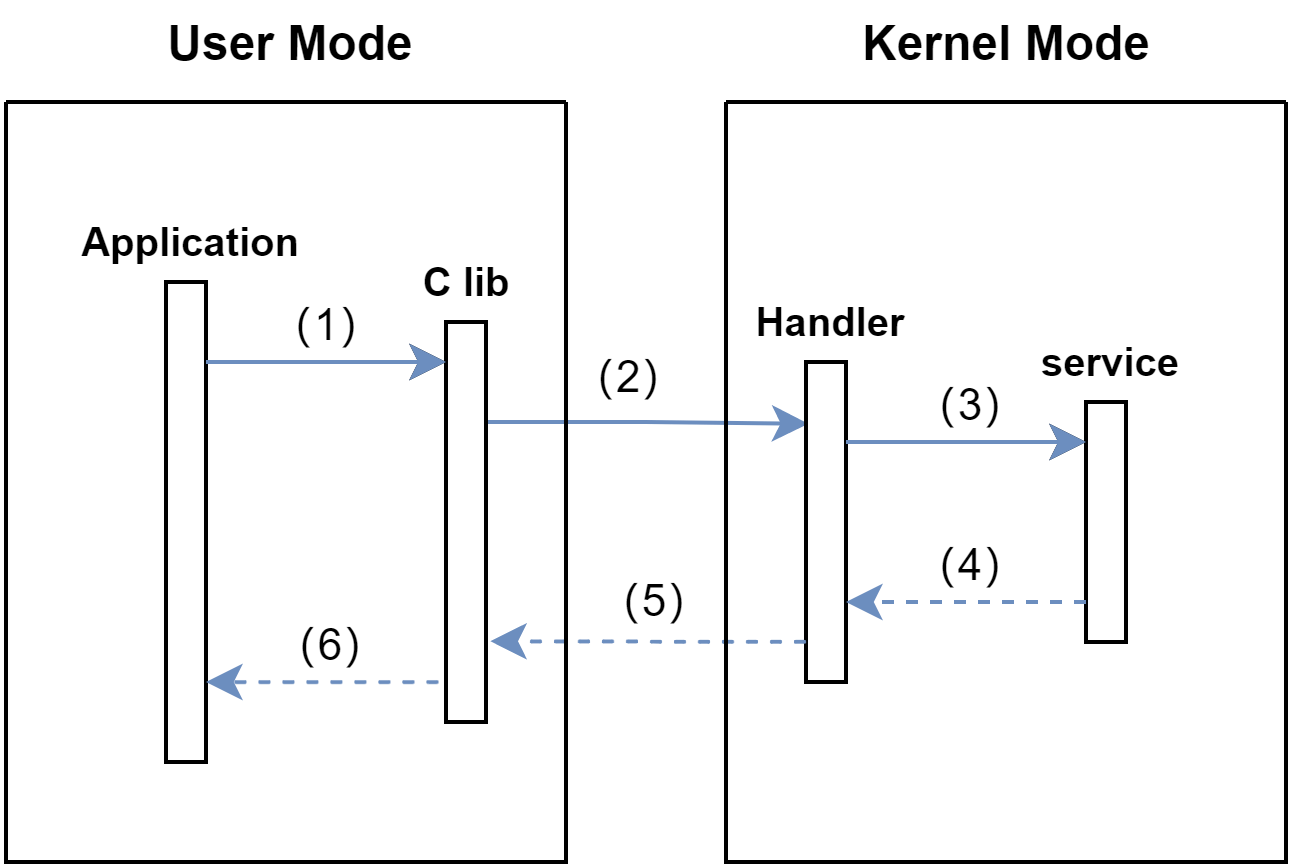
\includegraphics[width=0.8\textwidth]{images/system_call_process}
  \caption[Short description]{Systemc Call Process}
  \label{fig:system_call_process}
\end{figure}

After we understand how privileges are converted, let us now look at the process of a 
system call. As can see in figure ~\ref{fig:system_call_process}, a system call is invoked in most cases by going 
through a wrapper function (Step 1) in the C standard library. After the wrapper function 
traps the kernel into kernel mode via SYSCALL, the CPU jumps to the OS system-call handler 
function to continue executing(step 2). In this function, user stack and page-table are 
replaced by kernel stack and page table, respectively; the corresponding system call 
parameters are retrieved from proper registers, the value of all registers is saved 
on the kernel stack for construction of $struct pt_regs$ as some system calls like fork() 
need to have all registers on the stack. Finally, the OS system call handler (step3) calls 
the specific kernel service, and the result is returned to the user program in reverse order(step4-6).

Why is the system call process a performance issue? Compared to the function call, 
the caller and callee are in the same userspace. Almost every system call needs two 
context switches every time. 
This means that the context belonging to a running process needs to be saved to 
memory,  then replaced by the kernel's context. The more serious problem comes from 
cache miss, such as cache miss in TLB. TLB stands for Translation Lookaside Buffer 
that contains the virtual address to physical address mapping most likely to be 
accessed currently. Cache misses in the TLB can cause page faults, leading to 
significant performance penalties since the operating system will try to transfer 
the relevant page from the hard disk into the memory if the operating system 
determines that the page fault is valid. In addition, OS needs to do various 
checks during the privilege transition. All of those need time.

Nowadays as new hardware such as NVMe-based SSDs or RDMA network 
cards is put into use, The performance improvement of device is 
extremely obvious, e.g, the access delay is only a few microseconds, 
and the bandwidth can reach gigabytes per second.\cite{Yuhong}. 
Experiments show that when using a new generation of intelligent 
hardware, half of the overhead of one IO operation comes from the 
kernel software \cite{Yuhong}, because each IO operation requires 
two context switches, multiple copy operations between the device 
and user space, and may suffer multiple cache miss. Hence,  
the software is becoming a bottleneck of performance for IO operations.

In summary, five things that may lead to performance loss as system call enter or exit the kernel:

\begin{itemize}
  \item CPU context switch.
  \item The stack is switched from the user mode to the kernel mode, and the relevant information is stored in the kernel stack.
  \item User/kernel page table switch, and retrieve some pages needed by the kernel from Disk.
  \item Data caches and TLB invalidation after privilege transition caused by different run time environments between kernel and userspace.
   \item Multiple copy operations required between user and device through kernel.
\end{itemize}
\cleardoublepage

%%% Local Variables:
%%% TeX-master: "diplom"
%%% End:
